\section{Profil utilisateur}
\label{sec:profil}

La gestion de compte utilisateur ne semble pas être un élément essentiel pour une plateforme qui propose juste de consulter des documents de presse ancienne. Cependant, elle apporte tout de même un réel avantage concernant les revues de presse.
S'il n'y a pas de compte utilisateur et que l'utilisateur veut ajouter un article à une revue de presse, il devra à chaque fois rechercher la revue dans la base de données.
La présence de compte utilisateur va permettre de relier les revues de presse à un créateur et des contributeurs. Ainsi, les utilisateurs retrouveront la liste des revues créées et contribuées lorsqu'ils voudront ajouter l'article qu'ils sont en train de visualiser, à une revue.


\subsection{Apports}
\label{apport}
 

Un utilisateur qui disposera d'un compte aura accès à plusieurs fonctionnalités :

\begin{itemize}
  \item Avoir un compte utilisateur permet de créer des revues de presse ainsi que d'ajouter des articles aux revues et, si on en est le créateur, d'en enlever.
  \item Un ajout plus rapide d'un article à une revue qu'on a créée ou contribuée.
  \item Marquer des articles afin de pouvoir les retrouver facilement si l'utilisateur voudrait les relire plus tard. Ces articles seront rangés dans une revue de presse appelée "Articles favoris". Cette revue sera privée, c'est-à-dire que les autres utilisateurs ne pourront y accéder d'aucune façon. Les articles pourront aussi être enlevés par le propriétaire de la revue.
	\item Ajouter ou supprimer des annotations sur les articles.
\end{itemize}

En revanche, il n'est pas obligatoire d'avoir un compte utilisateur. Une personne qui n'a pas de compte peut tout de même rechercher un article ou une revue dans la base de données. Elle pourra aussi visualiser les documents ainsi que consulter les revues de presse. Mais elle ne pourra pas créer une revue de presse ni y ajouter des articles.


\subsection{Création d'un compte}
\label{creation_compte}


La création de compte se fera de la même manière que font d'ores et déjà la majorité des sites web. L'utilisateur devra entrer un pseudonyme, une adresse mail et un mot de passe. Il recevra ensuite un mail afin de confirmer la création du compte. La présence de l'adresse mail permettra de surcroît d'avoir une fonctionnalité "mot de passe oublié ?" permettant à l'utilisateur de pouvoir mettre un nouveau mot de passe pour son compte s'il a oublié le mot de passe courant.


\subsection{Espace utilisateur}
\label{espace_util}

\textit{voir ci-dessous Espace utilisateur et Paramètres}


Lorsque l'utilisateur est connecté, il pourra accéder à un espace utilisateur. Dans cet espace, l'utilisateur pourra voir la liste des articles qu'il a marqué. Cette liste sera sous forme de menu déroulant. Une partie des articles seront affichés mais l'utilisateur pourra voir le reste de la liste en cliquant sur les flèches qui se trouvent de part et d'autre du menu. Pour chaque article, il sera indiqué le titre de l'article, le nom du journal et la date ainsi que le début de l'article. En cliquant sur l'un des articles de la liste, l'utilisateur arrivera sur la page de visualisation de l'article.
Il aura aussi accès à la liste des revues qu'il a créées et celle des revues auxquelles il a contribuées. Ces listes se présenteront de la même façon que pour la liste des articles marqués. Pour chaque revue, le nom de la revue de presse sera indiqué. L'utilisateur pourra aller sur la page d'une des revues de presse en cliquant dessus.
Il y aura aussi un lien pour pouvoir créer une nouvelle revue de presse. 
Enfin, un lien vers les paramètres du compte sera présent.  Sur cette page, l'utilisateur pourra changer son mot de passe ainsi que son adresse mail.

    \begin{figure}[H]
        \centering
        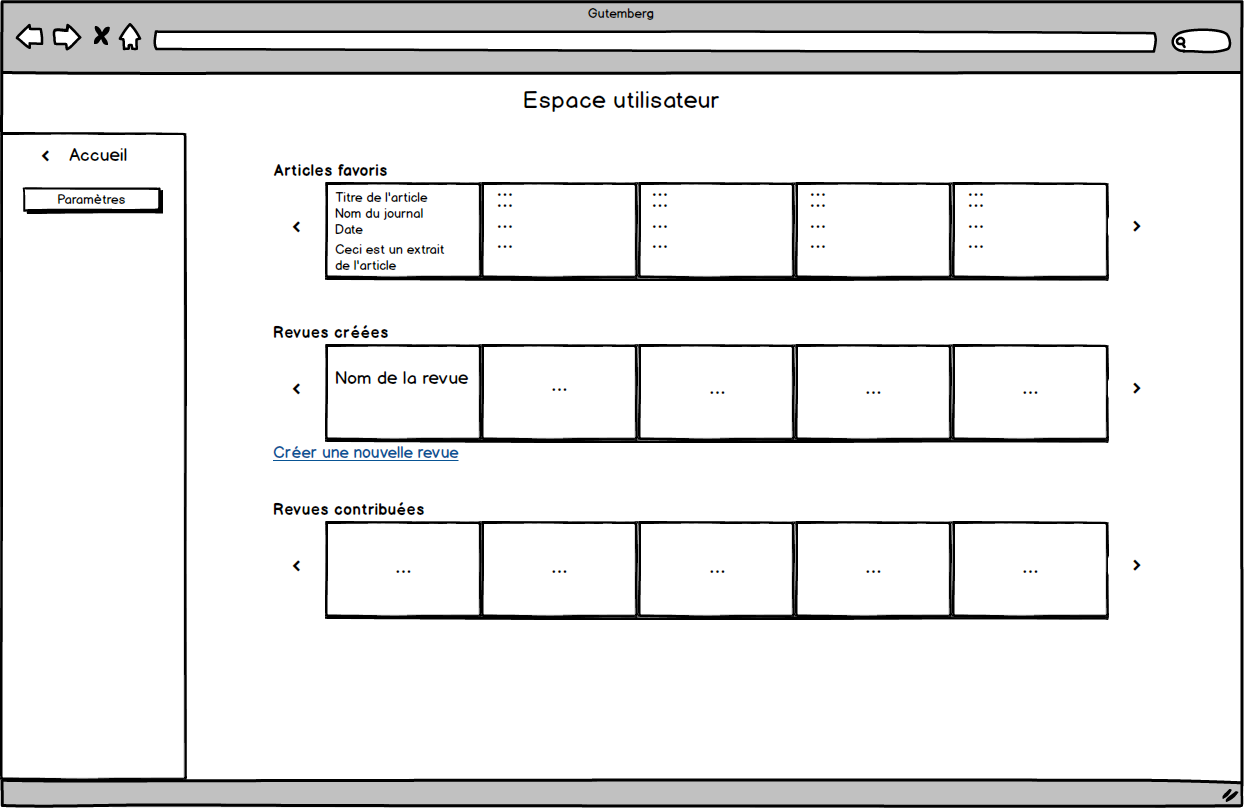
\includegraphics[width=\textwidth]{figures/Utilisateur.png}
            \caption{Page d'un profil utilisateur}
            \label{fig:utilisateur}
    \end{figure}

    \begin{figure}[H]
        \centering
        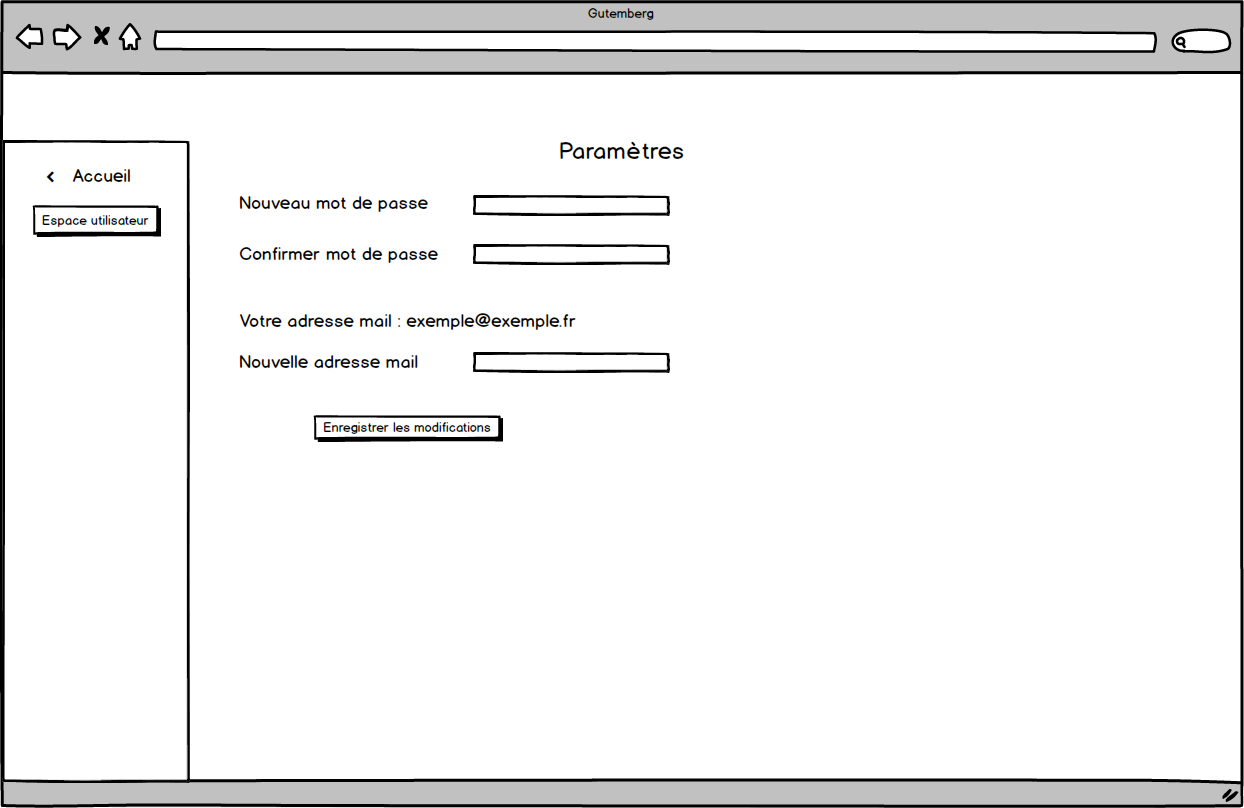
\includegraphics[width=\textwidth]{figures/Parametre.png}
            \caption{Paramètres utilisateur}
            \label{fig:utilisateur_parametre}
    \end{figure}